\documentclass{article} % Use article class for general formatting
\usepackage{pgfplots} % Include PGFPlots package
\pgfplotsset{compat=1.17} % Ensure compatibility with a modern version

\begin{document}
	
	\title{Your Paper Title Here}
	\author{Your Name \\ Your Affiliation \\ Your Email}
	\maketitle
	
	\begin{abstract}
		This is the abstract of your paper.
	\end{abstract}
	
	\section{Introduction}
	This is the introduction section of your paper.
	
	\section{Heatmap Example}
	Below is an example of a heatmap generated using PGFPlots in LaTeX:
	
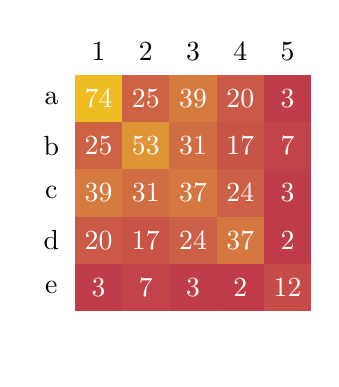
\begin{tikzpicture}[scale=0.6]
	\foreach \y [count=\n] in {
		{74,25,39,20,3},
		{25,53,31,17,7},
		{39,31,37,24,3},
		{20,17,24,37,2},
		{3,7,3,2,12},
	} {
		% column labels
		\ifnum\n<6
		\node[minimum size=6mm] at (\n, 0) {\n};
		\fi
		% heatmap tiles
		\foreach \x [count=\m] in \y {
			\node[fill=yellow!\x!purple, minimum size=6mm, text=white] at (\m,-\n) {\x};
		}
	}
	
	% row labels
	\foreach \a [count=\i] in {a,b,c,d,e,} {
		\node[minimum size=6mm] at (0,-\i) {\a};
	}
\end{tikzpicture}
	
	\section{Conclusion}
	This is the conclusion of your paper.
	
\end{document}
